% Options for packages loaded elsewhere
\PassOptionsToPackage{unicode}{hyperref}
\PassOptionsToPackage{hyphens}{url}
\PassOptionsToPackage{dvipsnames,svgnames,x11names}{xcolor}
%
\documentclass[
  letterpaper,
  DIV=11,
  numbers=noendperiod]{scrartcl}

\usepackage{amsmath,amssymb}
\usepackage{iftex}
\ifPDFTeX
  \usepackage[T1]{fontenc}
  \usepackage[utf8]{inputenc}
  \usepackage{textcomp} % provide euro and other symbols
\else % if luatex or xetex
  \usepackage{unicode-math}
  \defaultfontfeatures{Scale=MatchLowercase}
  \defaultfontfeatures[\rmfamily]{Ligatures=TeX,Scale=1}
\fi
\usepackage{lmodern}
\ifPDFTeX\else  
    % xetex/luatex font selection
\fi
% Use upquote if available, for straight quotes in verbatim environments
\IfFileExists{upquote.sty}{\usepackage{upquote}}{}
\IfFileExists{microtype.sty}{% use microtype if available
  \usepackage[]{microtype}
  \UseMicrotypeSet[protrusion]{basicmath} % disable protrusion for tt fonts
}{}
\makeatletter
\@ifundefined{KOMAClassName}{% if non-KOMA class
  \IfFileExists{parskip.sty}{%
    \usepackage{parskip}
  }{% else
    \setlength{\parindent}{0pt}
    \setlength{\parskip}{6pt plus 2pt minus 1pt}}
}{% if KOMA class
  \KOMAoptions{parskip=half}}
\makeatother
\usepackage{xcolor}
\setlength{\emergencystretch}{3em} % prevent overfull lines
\setcounter{secnumdepth}{-\maxdimen} % remove section numbering
% Make \paragraph and \subparagraph free-standing
\ifx\paragraph\undefined\else
  \let\oldparagraph\paragraph
  \renewcommand{\paragraph}[1]{\oldparagraph{#1}\mbox{}}
\fi
\ifx\subparagraph\undefined\else
  \let\oldsubparagraph\subparagraph
  \renewcommand{\subparagraph}[1]{\oldsubparagraph{#1}\mbox{}}
\fi


\providecommand{\tightlist}{%
  \setlength{\itemsep}{0pt}\setlength{\parskip}{0pt}}\usepackage{longtable,booktabs,array}
\usepackage{calc} % for calculating minipage widths
% Correct order of tables after \paragraph or \subparagraph
\usepackage{etoolbox}
\makeatletter
\patchcmd\longtable{\par}{\if@noskipsec\mbox{}\fi\par}{}{}
\makeatother
% Allow footnotes in longtable head/foot
\IfFileExists{footnotehyper.sty}{\usepackage{footnotehyper}}{\usepackage{footnote}}
\makesavenoteenv{longtable}
\usepackage{graphicx}
\makeatletter
\def\maxwidth{\ifdim\Gin@nat@width>\linewidth\linewidth\else\Gin@nat@width\fi}
\def\maxheight{\ifdim\Gin@nat@height>\textheight\textheight\else\Gin@nat@height\fi}
\makeatother
% Scale images if necessary, so that they will not overflow the page
% margins by default, and it is still possible to overwrite the defaults
% using explicit options in \includegraphics[width, height, ...]{}
\setkeys{Gin}{width=\maxwidth,height=\maxheight,keepaspectratio}
% Set default figure placement to htbp
\makeatletter
\def\fps@figure{htbp}
\makeatother

\KOMAoption{captions}{tableheading}
\makeatletter
\makeatother
\makeatletter
\makeatother
\makeatletter
\@ifpackageloaded{caption}{}{\usepackage{caption}}
\AtBeginDocument{%
\ifdefined\contentsname
  \renewcommand*\contentsname{Table of contents}
\else
  \newcommand\contentsname{Table of contents}
\fi
\ifdefined\listfigurename
  \renewcommand*\listfigurename{List of Figures}
\else
  \newcommand\listfigurename{List of Figures}
\fi
\ifdefined\listtablename
  \renewcommand*\listtablename{List of Tables}
\else
  \newcommand\listtablename{List of Tables}
\fi
\ifdefined\figurename
  \renewcommand*\figurename{Figure}
\else
  \newcommand\figurename{Figure}
\fi
\ifdefined\tablename
  \renewcommand*\tablename{Table}
\else
  \newcommand\tablename{Table}
\fi
}
\@ifpackageloaded{float}{}{\usepackage{float}}
\floatstyle{ruled}
\@ifundefined{c@chapter}{\newfloat{codelisting}{h}{lop}}{\newfloat{codelisting}{h}{lop}[chapter]}
\floatname{codelisting}{Listing}
\newcommand*\listoflistings{\listof{codelisting}{List of Listings}}
\makeatother
\makeatletter
\@ifpackageloaded{caption}{}{\usepackage{caption}}
\@ifpackageloaded{subcaption}{}{\usepackage{subcaption}}
\makeatother
\makeatletter
\@ifpackageloaded{tcolorbox}{}{\usepackage[skins,breakable]{tcolorbox}}
\makeatother
\makeatletter
\@ifundefined{shadecolor}{\definecolor{shadecolor}{rgb}{.97, .97, .97}}
\makeatother
\makeatletter
\makeatother
\makeatletter
\makeatother
\ifLuaTeX
  \usepackage{selnolig}  % disable illegal ligatures
\fi
\IfFileExists{bookmark.sty}{\usepackage{bookmark}}{\usepackage{hyperref}}
\IfFileExists{xurl.sty}{\usepackage{xurl}}{} % add URL line breaks if available
\urlstyle{same} % disable monospaced font for URLs
\hypersetup{
  pdftitle={Hierarchical mixing},
  colorlinks=true,
  linkcolor={blue},
  filecolor={Maroon},
  citecolor={Blue},
  urlcolor={Blue},
  pdfcreator={LaTeX via pandoc}}

\title{Hierarchical mixing}
\author{}
\date{}

\begin{document}
\maketitle
\ifdefined\Shaded\renewenvironment{Shaded}{\begin{tcolorbox}[enhanced, interior hidden, borderline west={3pt}{0pt}{shadecolor}, frame hidden, breakable, boxrule=0pt, sharp corners]}{\end{tcolorbox}}\fi

In \textbf{?@sec-MossGmelb}, we observed the construction of a
meta-population mixing matrix from empirical origin-destination (OD)
data. The patches used in the example were based on the `SA3' regions of
the Australian Statistical Geography Standard's Statistical Areas (SA)
classification {[}@2023AustralianStatisticalGeographya{]} (comprising 40
patches for the Greater Melbourne area in that example). In this chapter
we will use the larger ASGS SA classification structure to create
multiple meta population models of the same geographical area at
different spatial resolutions.

\hypertarget{hierarchical-structure-of-the-sa-classification}{%
\subsection{Hierarchical Structure of the SA
classification}\label{hierarchical-structure-of-the-sa-classification}}

An important feature of the SA classification structure is that there
are multiples scales of classification organised such that lower level
SAs are nested within higher level SAs. These levels are denoted by the
numbers 1-5, with special groupings for capital city areas
Figure~\ref{fig-ASGS}. For example, several SA3 regions can reside
within a single SA4 region, and multiple SA4 regions are contained
within the Greater Melbourne Capital City SA (GMCCSA). Moreover, each
SA3 region is partitioned into a number of SA2 scale regions, which in
turn are partitioned further into a number of SA1 scale regions.
Figure~\ref{fig-GMelbSA2SA3SA4} shows the borders of the 361 SA2, 40
SA3, and 9 SA4 regions of the GMCCSA.

\begin{figure}

{\centering 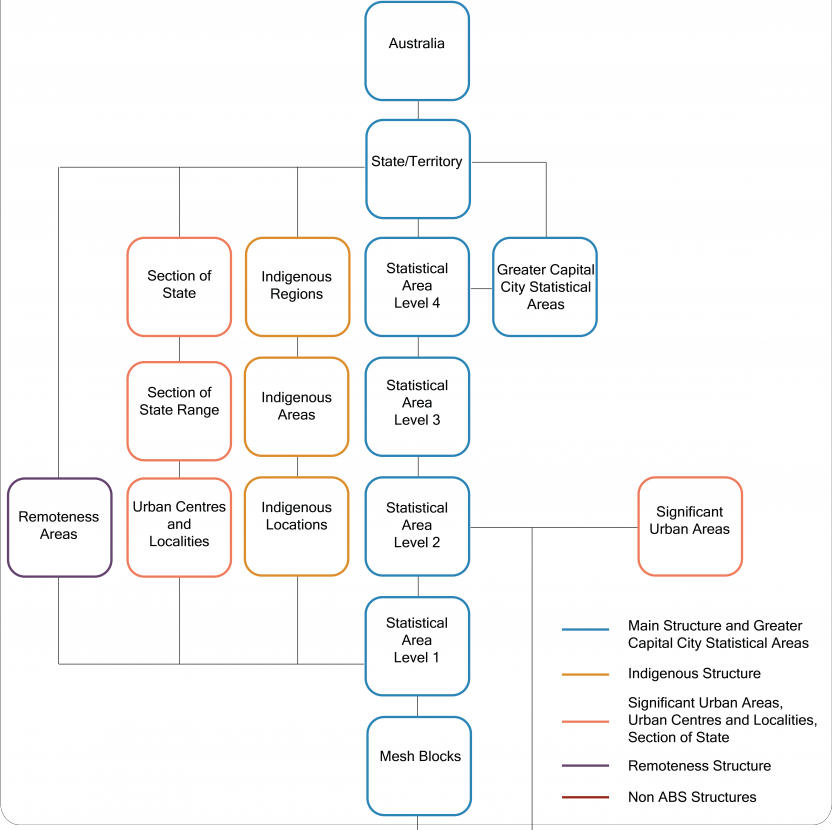
\includegraphics[width=4.16667in,height=\textheight]{figures/ASGS_Diagram_2021.png}

}

\caption{\label{fig-ASGS}Structure of The Australian Statistical
Geography Standard (ASGS) Statistical Areas (SA) Classification}

\end{figure}

For a specific example, the \texttt{Maribyrnong} SA3 region sits inside
the \texttt{West\ Melbourne}SA4 region alongside \texttt{Essendon} SA3
\textbf{?@fig-FootscraySAexample}. Both \texttt{West\ Melbourne} and the
neighbouring \texttt{Inner\ Melbourne} SA4 (containing the city center
and other SA3 regions), are part of the GSCCSA. Moreover, within
\texttt{Marybirnong} SA3 there are six SA2 level regions
(\texttt{Braybrook}, \texttt{Footscray}, \texttt{Maribyrnong},
\texttt{Seddon\ -\ Kingsville}, \texttt{West\ Footscray\ -\ Tottenham},
\texttt{Yarraville}), which can likewise be partitioned in to smaller
SA1 level and `Mesh Block' level regions Figure~\ref{fig-ASGS}. In
\textbf{?@fig-FootscraySAexample}, we highlight the SA1-SA4 level
regions containing the main Footscray CBD (SA1 code `21303134811'; see
Figure~\ref{fig-FootscraySA1Code}).

:::

Note that each red-bounded area represents a higher resolution (`lower'
SA level) than the one that encloses it.

\begin{figure}

\begin{minipage}[t]{0.50\linewidth}

{\centering 

SA2, SA3 and SA4 borders of the Greater Melbourne Greater Capital City
Statistical Area (GMGCCSA) and the the five SA3 blocks that make up the
`Melbourne - West' SA4 region, the six SA2 blocks that make up the
Maribyrnong SA3 region, the forty SA1 regionsa that make up the
`Footscray' SA2 region, and the sixteen mesh blocks that make up the
central Footscray `21303134811' SA1 region.

}

\end{minipage}%

\caption{\label{fig-GMelbSA2SA3SA4}\textbf{?(caption)}}

\end{figure}

Helpfully, besides a common name Statistical Areas are also indexed by a
structured code representing their classification hierarchy. For
example, SA1 regions are denoted by an 11 digit code which can be
decomposed into the higher level areas in which the region sits.
Figure~\ref{fig-FootscraySA1Code} demonstrates this for the Footscray
SA1 region considered above.

\begin{figure}

{\centering 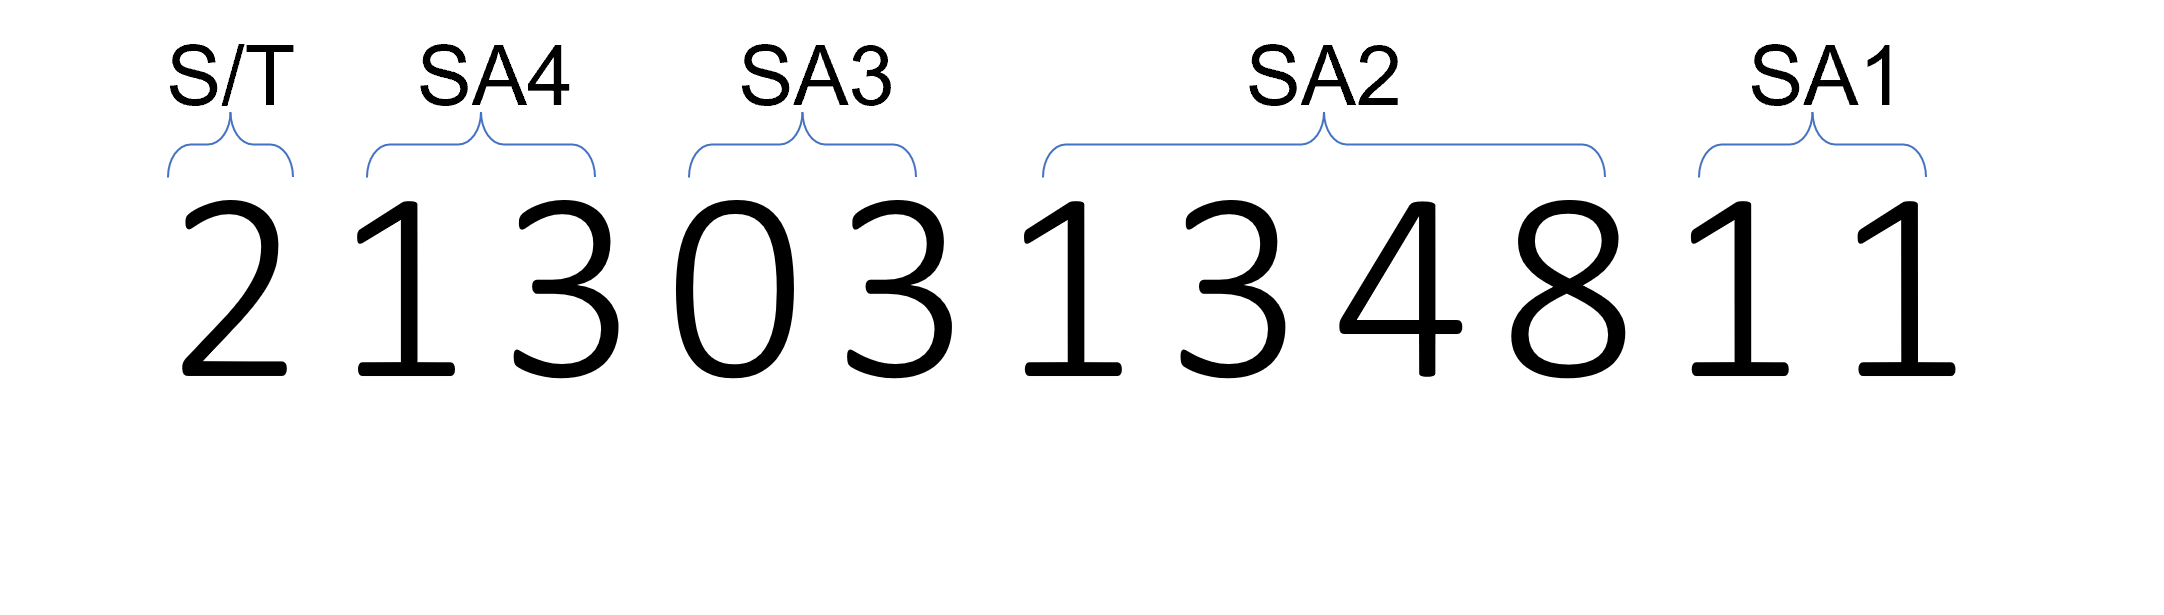
\includegraphics[width=2.58333in,height=\textheight]{figures/FootscraySA1eg.png}

}

\caption{\label{fig-FootscraySA1Code}Decomposition of theFootscray SA1
region code from \textbf{?@fig-FootscraySAexample} into its hierachical
SA components. 2 - \texttt{Victoria}; 13 - \texttt{West\ Melbourne}; 03
- \texttt{Maribyrnong}; 1348 - \texttt{Footscray}.}

\end{figure}

\hypertarget{comparisons-between-models-of-different-scales}{%
\subsection{Comparisons between models of different
scales}\label{comparisons-between-models-of-different-scales}}

\begin{itemize}
\item
  Spatial Epidemic models derived from empirical data are usually
  limited by the spatial resolution of their source material.
\item
  Comparing models at different scales has been achieved by using
  different model types (e.g.~agent based and compartental models) to
  represent different scales, (Or different parameterisations(?ref)
\item
  We can exploit the hierarchical structure of the ASGS Statistical
  Areas structure by creating meta-population models representing the
  same overarching spatial structure), but with varying levels of
  resolution (e.g.~by using SA2 scale patches instead of SA3 scale
  patches).
\item
  In what follows, we present metapopulation models of the GMGCSSA with
  patches corresponding to different levels of the SA hierarchy.
\end{itemize}

\hypertarget{homogenous-mixing-in-metapopulation-models}{%
\subsubsection{Homogenous mixing in metapopulation
models}\label{homogenous-mixing-in-metapopulation-models}}

We might initially consider the models with patch sizes 2, 3, 4 (for
SA2, SA3, SA4), and construct a mixing matrix with uniform mixing across
patches, i.e.~\[
m_{ij} = \frac{1}{n}
\]Where \(n\) is the total number of patches. While this mixing matrix
would entail homogeneous mixing in a metapopulation where
\(N_i = N_j, \forall i,j\), we have seen in
\textbf{?@fig-SA3Gmelb\_popn}, and as shown in
\textbf{?@fig-SA2Gmelb\_popn}, population size is not homogenous in the
GMGCCSA metapopoulations under consideration.

\hypertarget{sec-propmix}{%
\subsubsection{Proportionate mixing}\label{sec-propmix}}

To correct for hetrogeneous patch populations, We can scale mixing
coefficients by their patch size i.e.~for two patches \(i\) and \(j\)
the mixing coefficient \(\phi_{i,j}\):

\[
\phi_{ij} = N_j/N_{tot}
\]

Which gives mixing matrices shown in \textbf{?@fig-GMGCC\_PMM}

\begin{figure}

\begin{minipage}[t]{0.50\linewidth}

{\centering 

\raisebox{-\height}{

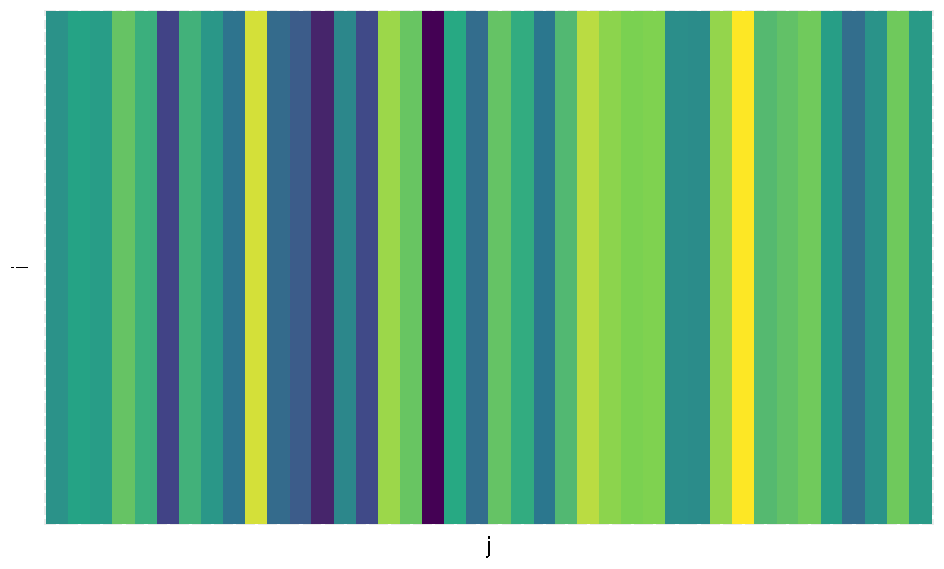
\includegraphics{Hmods_files/figure-pdf/fig-GMelb_PPM-1.pdf}

}

\caption{\label{fig-GMelb_PPM-1}SA3}

}

\end{minipage}%
%
\begin{minipage}[t]{0.50\linewidth}

{\centering 

\raisebox{-\height}{

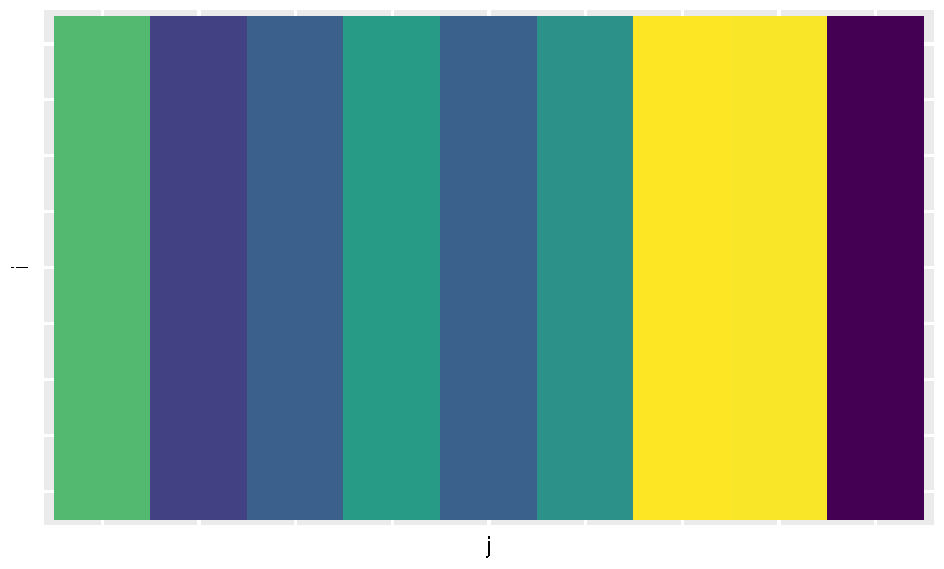
\includegraphics{Hmods_files/figure-pdf/fig-GMelb_PPM-2.pdf}

}

\caption{\label{fig-GMelb_PPM-2}SA4}

}

\end{minipage}%

\end{figure}

-total size -peak size -Duration of pop prop models with SA2 SA3 SA4
homogeneous patches - Expect equivalence

\hypertarget{sec-SAmixmat}{%
\subsubsection{Statistical Area Mixing structure}\label{sec-SAmixmat}}

We can encode the hierarchical structure of the SA classification in
hierarchical block matrices representing within and between SA region
mixing. To do so, we specify a set of coefficients
\(\xi = [\xi_1, ..., \xi_i]\) such that \(\sum\limits_{i}\xi_{i}=1\),
which determine the proportion of mixing occurs at each level, \(L\), of
the spatial hierarchy (i.e.~between SA2 regions, between SA3 regions,
etc.) . This coefficient is distributed amongst patches occurring in the
same level \(L\) region, so mixing for any two patches, \(i\) and \(j\)
\begin{equation}\protect\hypertarget{eq-SAmix}{}{
M_{ij}= \frac{\xi_{L}}{n^{L}} 
}\label{eq-SAmix}\end{equation} where \[
j \in S_{i}^{L} \  \& \ j \notin S_{i}^{L-1}
\] and \(S_{i}^{L}\) is the set of patches in the same level \(L\)
region as \(i\).

To extend the example from \textbf{?@sec-XX}, we can consider a subset
of SA2 regions from the GMGCCSA (\textbf{?@fig-GMelb\_eg\_Map},
@tab-MMeg)

Docklands and West industrial are SA2 regions within the `Melbourne
City' SA3 region. Port Melbourne and Port Industrial are SA2 regions
within the `Port Melbourne' SA3 region. Footscray, Seddon-Kingsville,
and Yarraville are SA2 regions within the `Maribyrnong' SA3 region.
Newport SA2 is within the Hobsons Bay SA3 region. Port Melbourne and
Port Industrial are SA2 regions within the `Port Melbourne' SA3 region.
Furthermore, both `Melbourne city' and `Port Melbourne' are within the
`Inner Melbourne' SA4 region, while Maribyrnong and Hobsons Bay SA3 lie
inside the `West Melbourne' SA4 Region.

To model mixing between these SA2 patches (isolated from the rest of the
GMGCCSA), we can construct a \(8 \times 8\) mixing matrix with
\(\xi = \left[ \frac{1}{4}, \frac{1}{4},\frac{1}{4},\frac{1}{4} \right]\)
as follows:

let \(i =\) \texttt{Footscray}. Since \texttt{Footscray} is it's own SA2
region, \[M_{i,i} = \frac{1}{4}\] When \(j\) is a region in
\texttt{Maribyrnong} SA3 (alongside \texttt{Footscray}), like
\texttt{Yarraville} or \texttt{Seddon-Kingsville}, \(M_{i,j}\) will be a
proportion of \(\xi_{SA3}\). \[
M_{i,j} = \frac{\xi_{SA3}}{P_{i}^{SA3} - P_{i}^{SA2}} = \frac{\frac{1}{4}}{3 - 1} = \frac{1}{8}
\] When \(j\) occurs outside the \texttt{Maribyrnong} SA3, but within
the \texttt{West\ Melbourne} SA4, like \texttt{Newport} SA2 \[
M_{i,j} = \frac{\xi_{SA4}}{P_{i}^{SA4} - P_{i}^{SA3}} = \frac{\frac{1}{4}}{4 - 3} = \frac{1}{4}
\] Finally when \(j\) is a patch outside the \texttt{West\ Melbourne}
SA4, like those in the \texttt{Inner\ Melbourne}SA4 \[
M_{i,j} = \frac{\xi_{SA5}}{P_{i}^{SA5} - P_{i}^{SA4}} = \frac{\frac{1}{4}}{8 - 4} = \frac{1}{16}
\] thus for the row \(M_{i}\), representing the mixing of individuals
from Footscray,
\(\sum\limits_{j}M_{j}= \frac{1}{4} +\frac{1}{8} + \frac{1}{8} + \frac{1}{4} + \frac{1}{16} + \frac{1}{16} + \frac{1}{16} + \frac{1}{16} = 1\).
Repeating this for all patches \(i\), gives the mixing matrix
represented in \textbf{?@fig-GMelb\_eg\_MixMat}

\begin{figure}

\begin{minipage}[t]{0.50\linewidth}

{\centering 

\raisebox{-\height}{

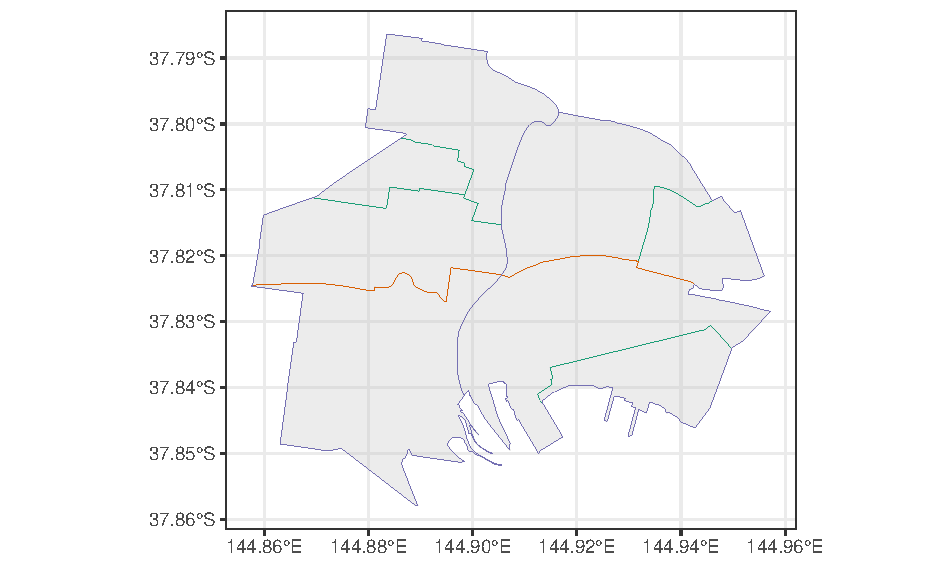
\includegraphics{Hmods_files/figure-pdf/fig-GMelb_eg-1.pdf}

}

\caption{\label{fig-GMelb_eg-1}A}

}

\end{minipage}%
%
\begin{minipage}[t]{0.50\linewidth}

{\centering 

\raisebox{-\height}{

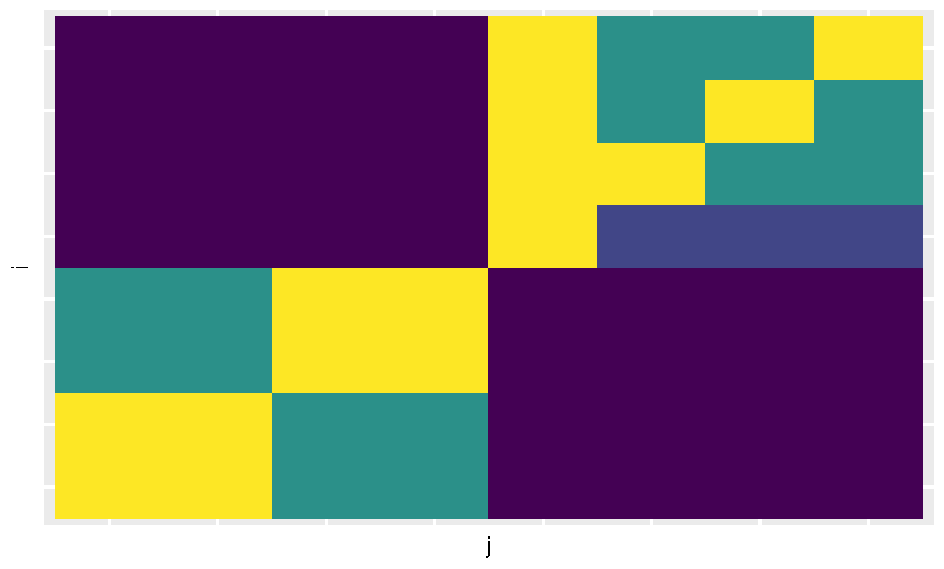
\includegraphics{Hmods_files/figure-pdf/fig-GMelb_eg-2.pdf}

}

\caption{\label{fig-GMelb_eg-2}B}

}

\end{minipage}%

\end{figure}

Applying this process to the whole GMGCCSA yields the mixing matrices
presented in figure \textbf{?@fig-GCC\_HMM}

\begin{figure}

\end{figure}

Hierarchical Mixing matrices for the Greater Melbourne Capital City
Statistical Area (GMGCCSA) at three levels of spatial resolution.

\hypertarget{population-normalised-sa-mixmat}{%
\subsubsection{Population normalised SA
mixmat}\label{population-normalised-sa-mixmat}}

\begin{figure}

\end{figure}

\begin{itemize}
\item
  in the same way as in \textbf{?@sec-proportionatemixing}, the SA
  structured mixingmatrix given in Section~\ref{sec-SAmixmat},
  Equation~\ref{eq-SAmix}, will result in hetrogenous mixing due to the
  different population per patch \textbf{?@fig-gmelbpop}.
\item
  Again, we can rectify this by scaling columns in the mixing matrix by
  the according population size. Due to the hierarchical structure we
  can reduce patch counts to population counts
\end{itemize}

\[M_{ij} = \frac{N_{j}}{N_{i}^{L} - N_{i}^{L-1}} \xi^{L}\] if
\(j \in S_{i}^{L}\) \& \(j \notin S_{i}^{L-1}\)

where \(i, j\) are patches \(S_{i}^{L}\) is the set of patches in level
\(L\) \(N_i\) is the population of \(i\) \(N_{i}^{L}\) is the population
of \(S_{i}^{L}\) \(\xi^{L}(\delta)\) is the proportion of mixing that
occurs within \(S_{i}^{L}\) but not\(S_{i}^{L-1}\)

\begin{figure}

\begin{minipage}[t]{0.50\linewidth}

{\centering 

\raisebox{-\height}{

\includegraphics{Hmods_files/figure-pdf/fig-gmelbpop-1.pdf}

}

\caption{\label{fig-gmelbpop-1}fig-gmelbpop\_SA1}

}

\end{minipage}%
%
\begin{minipage}[t]{0.50\linewidth}

{\centering 

\raisebox{-\height}{

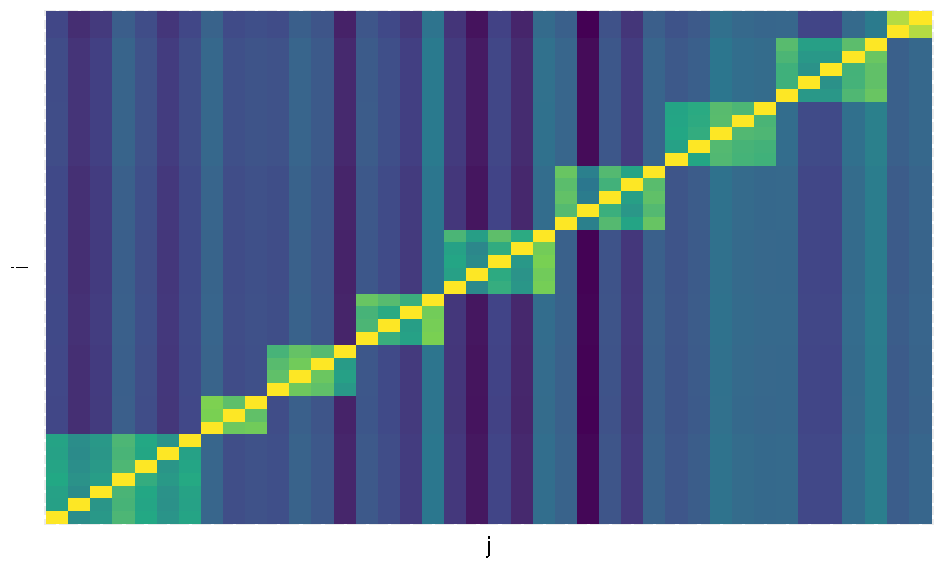
\includegraphics{Hmods_files/figure-pdf/fig-gmelbpop-2.pdf}

}

\caption{\label{fig-gmelbpop-2}fig-gmelbpop\_SA2}

}

\end{minipage}%
\newline
\begin{minipage}[t]{0.50\linewidth}

{\centering 

\raisebox{-\height}{

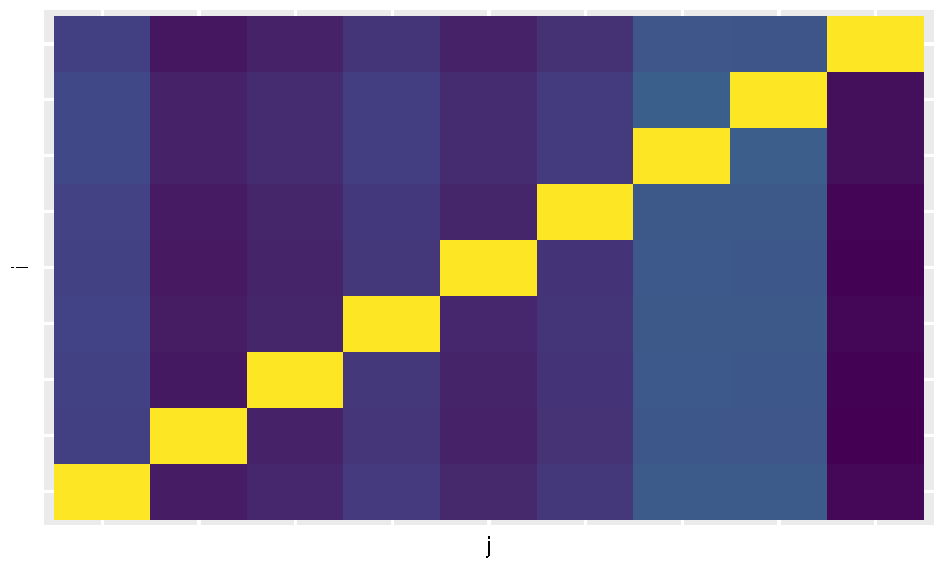
\includegraphics{Hmods_files/figure-pdf/fig-gmelbpop-3.pdf}

}

\caption{\label{fig-gmelbpop-3}fig-gmelbpop\_SA3}

}

\end{minipage}%

\end{figure}

\hypertarget{simulation}{%
\subsubsection{Simulation}\label{simulation}}

\begin{itemize}
\tightlist
\item
  We can now simulate the spread of a disease through the GMGCCSA using
  the mixing matrices presented in Section~\ref{sec-SAmixmat} and
  \textbf{?@sec-HPMM}.
\item
  We will use the same parameters as in \textbf{?@sec-sim}, but now we
  will use the population normalised mixing matrices.
\end{itemize}

\begin{figure}

\begin{minipage}[t]{0.50\linewidth}

{\centering 

Final (a) and peak (b) infection numbers (as a proportion of the entire
population), peak time (c) and total duration (d) of a simulated SIR
metapopulation model with OD mixing matrix at different values of
\(\delta^H\) and \(R_0\)

}

\end{minipage}%

\caption{\label{fig-SA3_OD_outcomes}\textbf{?(caption)}}

\end{figure}

However, now we can decompose these metapopulation scale outcomes into
those of the underlying subpopulation. For example,
\textbf{?@fig-OD\_patchinf\_curve\_eg}



\end{document}
